\chapter{Latent and Sensible Heat Flux Calculations over First-Year Sea Ice}
\vspace{1 cm}
\begin{spacing}{1} \begin{quote} 
\noindent \emph{A recent review of the latent and sensible heat flux accuracies over the period 2000–2007 highlights significant differences between several gridded products over ocean, where root-mean-squared differences between the multi-product ensemble and data at more than 200  moorings reached up to 25 $W m^{–2}$ for latent heat and 5 $W m^{–2}$ for sensible heat. This uncertainty stems from the retrieval of flux-relevant meteorological variables, as well as from differences in the flux parametrizations.} \end{quote}
\hspace{6 cm} - IPCC Sixth Assessment Report, August 2021  
\end{spacing}
\doublespacing
\section{Introduction}
% why is SEB important
It is important to fully understand the surface energy budget over sea ice because small changes in radiative and/or turbulent fluxes enact feedbacks that can result in significant climate impacts. Reductions in sea ice have been found to amplify the impacts of global warming \citep{wunderling:2020, ipcc_techsum}. Differences in the surface features and atmospheric conditions present challenges for modeling the surface energy and water budgets \citep{wang:2009}. 

\begin{equation}\label{eq:seb}
F_{s} - C = Q_{net} + H_{s} + H_{l}
\end{equation}

% what is the sensible and latent heat flux physically?
The surface energy budget can be seen in \ref{eq:seb}. The net radiative flux, $Q_{net}$, is the combination of the shortwave and longwave radiation (downward - upward), $F_{s}$ is the energy storage, and $C$ is the heat flux from the underlying ocean \citep{walden:2017}. The turbulent fluxes, $H_{s}$ and $H_{l}$, are the sensible and latent heat fluxes and are the focus of this chapter. Physically, the sensible heat flux represents conduction between the atmosphere and the surface that is driven by the temperature gradient near the surface. As defined here, positive sensible heat flux represents energy into the surface, which would occur when the near-surface atmospheric temperature is warmer than the surface. This is often the case during the winter when either near-surface temperature inversions occur or when warm air is advected over the frozen surface. Negative sensible heat flux values represent energy lost by the surface, which occurs when the surface is warmer than the overlying atmosphere. Latent heat flux is the heat associated with a phase change; positive latent heat flux is representative of deposition, condensation, or freezing at the surface, and negative latent heat occurs during sublimation, evaporation, or melting.

% measuring SEB
Some components of the surface energy budget, such as shortwave and longwave radiation, can be measured directly with radiometers. The sensible and latent heat flux, however, is more difficult to measure. A common approach is to use the Eddy Covariance technique. This is explained briefly by \citet{walden:2017}. First, high-frequency covariance measurements are made at different heights above the surface of temperature, wind speed and direction, and water vapor concentration. LiCor's EddyPro 7 \citep{epro} software is then used to process these measurements. The program conducts calibration and filtering on the raw measurements, then calculates the sensible and latent heat fluxes. the covariance measurements were made by a Campbell Scientific CSAT3 sonic anemometer and gas analyzer operated by researchers from the Norwegian Polar Institute. 

% field campaigns measuring the SEB
The Norwegian Young Sea Ice Field Campaign (N-ICE) in 2015 and the Surface Heat Budget of the Arctic Ocean Experiment (SHEBA) in 1998 both deployed eddy covariance (EC) systems, radiometers, and meteorological towers over sea ice in the Arctic ocean. SHEBA took place over older, multi-year sea ice, and the data collected has been processed both using EC theory and using other methods not requiring the EC system. N-ICE took place over young, first-year sea ice. A description of the turbulent fluxes observed by the EC system and the radiation measured by radiometers can be found in \citet{walden:2017}, which describes the observed surface energy budget at N-ICE. 

\section{Calculating Sensible and Latent Heat Flux}
In this section, the measured turbulent fluxes are compared to two methods of calculating sensible and latent heat flux: a bulk flux algorithm based on Monin-Obukhov similarity theory \citep{foken:2008} and the Maximum Entropy Production (MEP) method \citep{zhang:2021, wang:2014, wang:2009}. Both methods estimate flux without covariance measurements and instead utilize values more commonly observed at weather stations. The following subsection will give details about how the stability is used to calculate the stability-dependant scaling parameters required by equations for both the bulk flux algorithm and the MEP method.  

\subsection{Bulk Flux Algorithm}
The bulk flux algorithms are most commonly used for estimating turbulent fluxes \ref{reeves:2021} in models because they are relatively easy to calculate (depend only on meteorological variables) and are computationally efficient. The bulk flux algorithm formulations of sensible and latent heat flux used here are shown in Eq. \ref{eq:hs} and \ref{eq:hl} and are referred to as the "bulk flux algorithm" for the rest of this paper.

\begin{equation}\label{eq:hs}
H_{s} = \rho c_{p} C_{Hz} w [T_{s} - T_{z}]
\end{equation}
\begin{equation}\label{eq:hl}
H_{l} = \rho L_{v} C_{Ez} w [q_{s} - q_{z}] 
\end{equation}

Sensible and latent heat flux depend on measurements of wind speed potential temperature ($\theta_{s}$ and $\theta_{z}$) and specific humidity ($q_{s}$ and $q_{z}$) at the surface and a reference height, (for this case 2 $m$ and 4 $m$). In these equations, $\rho$ is the density of the air, $c_{p}$ the specific heat of air, $L_{v}$ the latent heat of vaporization, and $C_{hz}$ and $C_{Ez}$ are the heat and moisture exchange bulk transfer coefficients \citep{foken:2008, andreas:311}. Eq. \ref{eq:chz} and \ref{eq:cez} are the generally accepted functions for estimating these coefficients. 

\begin{equation}\label{eq:cez}
C_{Ez} = \frac{\kappa C_{D}^{\frac{1}{2}}}{[ln(\frac{z}{z_{0}})-\varphi_{h}]}
\end{equation}
\begin{equation}\label{eq:chz}
C_{hz} =  \kappa^{2} \left[ ln \left( \frac{z}{z_{0}} \right) - \varphi_{m} \right] ^{-1} \left[ ln \left( \frac{z}{z_{0}} \right) - \varphi_{h} \right] ^{-1}
\end{equation}

These equations are functions of $\varphi_{m}$ and $\varphi_{h}$, the scaling parameters, which depend on the surface stability. They also require estimations of the drag coefficient ($C_{D}$) and the roughness length ($z_{0}$).

\subsection{Maximum Entropy Production Method} 
The MEP method was developed to accurately estimate surface fluxes while limiting the number of empirically-derived values and scaling parameters used. This method is based on the principle of maximum entropy and Bayesian probability theory from statistical mechanics \citep{wang:2014}. Equations \ref{eq:mep:hl}, \ref{eq:mep:hs}, and \ref{eq:mep:rn} are the MEP formulations for sensible ($H_{s}$), latent ($H_{l}$), and surface thermal ($Q_{net}$) energy flux, respectively. 

\begin{equation}\label{eq:mep:rn}
\left[ 1 + B(\theta) + \frac{B(\theta_{pc})}{\theta_{pc}} \frac{I_{wsi}}{I_{0}} | H_{s} | ^{-\frac{1}{6}} \right] H_{s} = Q_{net}
\end{equation}
\begin{equation}\label{eq:mep:hl}
H_{l} = B(\theta_{pc}) H_{s}
\end{equation}
\begin{equation}\label{eq:mep:hs}
Q_{net} = Q_{lw} - H_{l} - H_{s}
\end{equation}

Eq. \ref{eq:mep:b} is required by both the sensible and latent heat flux calculations and needs an estimation of the phase change parameter ($\theta_{pc}$, defined in \citep{wang:2011} as Eq. 9). Calculations of sensible and latent heat flux using this method require estimations of the thermal conductivity \citep{wang:2014} of the surface. The thermal inertia parameter of the sea ice ($I_{wsi}$ \ref{eq:iwsi}) used in the MEP equation requires the air density ($\rho$), specific heat ($c_{p}$), and thermal conductivity or the surface ($\lambda$). \citet{merkouriadi:2017} found that the thermal conductivity of snow on sea ice during N-ICE2015 was much lower than those used in many modeling studies, so the thermal inertia parameter needs to be calculated for our location using an appropriate thermal conductivity value. 

\begin{equation}\label{eq:mep:b}
B(\theta_{pc}) = 6 \left( \sqrt{1 + \frac{11}{36} \theta_{pc}} - 1 \right)
\end{equation}
\begin{equation}\label{eq:iwsi}
I_{wsi} = \sqrt{\rho c_{p} \lambda}
\end{equation}
\begin{equation}\label{eq:i0}
I_{0} = \rho c_{p} \sqrt{C_{Ez}\kappa Z} \left( C_{Hz} \frac{\kappa Zg}{\rho c_{p} T_{r}} \right)^{\frac{1}{6}}
\end{equation}

$I_{0}$ can be calculated by \ref{eq:i0}. This value is called "the apparent thermal inertia of air" by \citet{wang:2009}. It depends on the heat and moisture exchange bulk transfer coefficients ($C_{hz}$ and $C_{ez}$), which are defined in the previous section. In this equation, $\kappa$ is the K\'{a}rm\'{a}n constant, $z$ is the measurements height (2 $m$ for this study), $g$ is the gravitational constant, and $T_{r}$ is a reference temperature of 300 $K$. 

This model has been used to calculate fluxes during SHEBA with some degree of accuracy, proving its ability to perform in the polar regions \citep{wang:2014}. Note that the sign convention for the sensible and latent heat fluxes for this formulation is opposite that given in \ref{eq:seb}, however, this is taken into account in all of the analyses performed here.

\subsection{Surface Stability}
Some commonly accepted sets of equations for the empirical scaling equations ($\varphi_{h}$ and $\varphi_{m}$ for $C_{hz}$ and $C_{ez}$) are shown in Table \ref{tab:stability}. These equations use the surface-layer stability parameter (Eq. \ref{eq:zl}) to determine surface stability. These values depend on the Obukhov length ($L$ Eq. \ref{eq:l}). Obukhov length requires estimations of the covariance of the wind velocity and virtual potential temperature ($\overline{w'\theta_{v}'}$), friction velocity ($u_{*}$), and the virtual potential temperature ($\theta_{v}$). 

\begin{equation}\label{eq:zl}
\zeta = \frac{z}{L}
\end{equation}
\begin{equation}\label{eq:l}
L = -\frac{u_{*}^{3}}{\kappa \frac{g}{\theta_{s}} \overline{w'\theta_{v}'}}
\end{equation} 

Positive surface-layer stability parameter numbers indicate stable conditions and negative indicate unstable conditions. Some studies find that using an adjusted von K\'{a}rm\'{a}n constant ($\kappa$) can improve calculations \citep{businger:1971, zilitinkevitsch:1968, dyer:1970}, but changing this variable is outside the scope of this study, so only formulations using $\kappa = 0.4$ to calculate $\zeta$ are included in Table \ref{tab:stability}. 

{
\begin{table*}[p]
\center
\centering
\scriptsize
    \begin{tabular}{| c | c |}
    \hline
        \rowcolor[HTML]{F3F3F3} \textbf{Author} & \textbf{Equations} \\ \hline
        \shortstack{Swainbank \\ \citep{foken:2008}} & \shortstack{$\varphi_{m} = \begin{cases} 0.613(-\zeta)^{-0.2} & \text{    } -0.1 \geq \zeta \geq -2 \\ \end{cases}$ \\ $\varphi_{H} = \begin{cases} 0.226 (-1/L)^{-0.44} & \text{    } -0.1 \geq \zeta \geq -2 \\ \end{cases}$} \\ 
        \hline
        \shortstack{Tschalikov \\ \citep{foken:2008}}  & \shortstack{$\varphi_{m} = \begin{cases} 1 + 7.74\zeta & \text{    } \zeta \geq 0.04 \\ \end{cases}$\\$\varphi_{H} = \begin{cases} 1 + 5.17\zeta & \text{    } \zeta \geq 0.04 \\ \end{cases}$ } \\ 
                \hline
                \shortstack{Zilitinkevich and \\ Tschalikov \\ \citep{zilitinkevitsch:1968}}  & \shortstack{$\varphi_{m} = \begin{cases} 1 + 1.38 \zeta & \text{    } -0.15 < \zeta < 0 \\ 0.42(-\zeta)^{1/3} & \text{    } -1.2 < \zeta < -0.15 \\ 1 + 9.4 \zeta & \text{    } 0 < \zeta \\ \end{cases}$\\$\varphi_{H} = \begin{cases} 1 + 1.31 \zeta & \text{    } -0.15 < \zeta < 0 \\ 0.41(-\zeta)^{-1/3} & \text{    } -1.2 < \zeta < -0.15 \\ 0.95 + 8.9 \zeta & \text{    } 0 < \zeta \\ \end{cases}$ } \\ 
                        \hline
        \shortstack{Businger et al. \\ \citep{businger:1971}}  & \shortstack{$\varphi_{m} \begin{cases} (1 - 19.3 \zeta)^{-1/4} & \text{    } -2 < \zeta < 0 \\ 1 + 6\zeta & \text{    } 0 < \zeta < 1 \\ \end{cases}$\\$\varphi_{H} \begin{cases} 0.95(1 - 11.6 \zeta)^{-1/2} & \text{    } -2 < \zeta < 0 \\ 0.95 + 7.8\zeta & \text{    } 0 < \zeta < 1 \\ \end{cases}$ } \\ 
                \hline
       \shortstack{Dyer \\ \citep{dyer:1974}} & \shortstack{$\varphi_{m} \begin{cases} (1 - 15.2 \zeta)^{-1/2} & \text{    } -1 < \zeta < 0 \\ 1 + 4.8\zeta & \text{    } 0 < \zeta \\  \end{cases}$ } \\ 
               \hline
        \shortstack{Skeib \\ \citep{foken:1990}} & \shortstack{$\varphi_{m} = \begin{cases} 1 & \text{    } -0.0625 < \zeta < 0.125 \\ (\frac{\zeta}{-0.0625})^{-1/4} & \text{    } -2 < \zeta < -0.0625 \\ \frac{\zeta}{0.125} & \text{    } 0.125 < \zeta < 2 \\ \end{cases}$\\$\varphi_{H} = \begin{cases} 1 & \text{    } -0.0625 < \zeta < 0.125 \\ 0.95(\frac{\zeta}{-0.0625})^{-1/2} & \text{    } -2 < \zeta < -0.0625 \\ 0.95(\frac{\zeta}{0.125})^{2} & \text{    } 0.125 < \zeta < 2 \\ \end{cases}$ } \\ 
              \hline
       \shortstack{Gavrilov and \\ Petrov \\ \citep{gavrilov:1981}}  & \shortstack{$\varphi_{m} = \begin{cases} (1-8\zeta)^{-1/3} & \text{    } \zeta < 0\\ 1 + 5 \zeta & \text{    } 0 < \zeta\\ \end{cases}$\\$\varphi_{H} = \begin{cases} 0.65 \left[ (1-35\zeta)^{-1/2} + \frac{0.25}{1+8(\zeta)^{2}} \right] & \text{    } \zeta < 0\\ 0.9 + 6 \zeta & \text{    } 0 < \zeta\\ \end{cases}$ } \\ 
               \hline
        \shortstack{Dyer and \\ Bradley \\ \citep{dyer:1982}}  & \shortstack{$\varphi_{m} = \begin{cases} (1 - 28\zeta)^{-1/4} & \text{    } \zeta < 0 \\ \end{cases}$\\$\varphi_{H} = \begin{cases} (1 - 14\zeta)^{-1/2} & \text{    } \zeta < 0 \\ \end{cases}$ } \\ 
                \hline
        \shortstack{Beljaars and \\ Holtslag \\ \citep{beljaars:1991}}  & \shortstack{$\varphi_{m} = \begin{cases} 1 + \zeta + \frac{2}{3} \zeta (6 - 0.35 \zeta) e^{-0.35} \zeta & \text{    } \zeta < 0 \\ \end{cases}$\\$\varphi_{H} = \begin{cases} 1 + \zeta + (1_+ \frac{2}{3} \zeta)^{1/2} (6 - 0.35 \zeta) e^{-0.35 \zeta} & \text{    } \zeta < 0 \\ \end{cases}$ } \\ 
                \hline
        \shortstack{Handorf et al. \\ \citep{handorf:1999}} & \shortstack{$\varphi_{m} = \begin{cases} 1 + 5 \zeta & \text{    } 0 < \zeta < 0.6 \\ 4 & \text{    } \zeta > 0.6 \\ \end{cases}$\\$\varphi_{H} = \begin{cases} 1 + 5 \zeta & \text{    } 0 < \zeta < 0.6 \\ 4 & \text{    } \zeta > 0.6 \\ \end{cases}$ } \\ 
              \hline
       \shortstack{Andreas et al. \\ \citep{andreas:2009}} & \shortstack{$\varphi_{m} = \begin{cases} BDP(\gamma = 16) & \text{    } \zeta < 0 \\ -5z/L & \text{    } \zeta \geq 0 \\ \end{cases}$ \\ $\varphi_{H} = \begin{cases} \varphi_{m}^{2} & \text{    } \zeta < 0 \\ \varphi_{m} & \text{    } \zeta \geq 0 \\ \end{cases}$ } \\ 
        \hline
    \end{tabular}
    \caption[Scaling parameter equations.]{Scaling parameter equations from Micrometeorology \citep{foken:2008} for the universal functions of momentum and heat. 'BDP' represents the Businger-Dyer-Pandolfo relationship, as seen in Eq. \ref{eq:bdp:H} and \ref{eq:bdp:m}. \citep{foken:2008}.}
    \label{tab:stability}
\end{table*}}

Each of the equations shown in the table have different ranges of stability to which they can be applied. These are formulated empirically, meaning they depend on measurements and are useful only under similar conditions \citep{stull:1988, foken:2008}. These equations were selected as they are those listed by \citet{foken:2008} in the book \textit{Micrometeorology} for use using the von K\'{a}rm\'{a}n constant equal to 0.4. One equation, the \citet{andreas:2010} formulation, was selected despite it being absent from the list in \citet{foken:2008}. Many of these equations, with the exception of \citet{andreas:2010}, were created under conditions observed in mid-latitudes. \citet{andreas:2010}, on the other hand, used results from the SHEBA field experiment to tune the relationships based on the Businger-Dyer-Pandolpho (BDP) relationship (Eq. \ref{eq:bdp:m} and \ref{eq:bdp:H}). This relationship is generally used for neutral and unstable conditions \citep{foken:2008}, so it requires tuning for other locations. Unlike many of the equations in Table \ref{tab:stability}, the BDP relationship requires an extra variable, $\gamma$, which is defined empirically for each location.

\begin{equation}\label{eq:bdp:m}
\varphi_{m}(\zeta) = (1 + \gamma \zeta)^{-1/4}
\end{equation}
\begin{equation}\label{eq:bdp:H}
\varphi_{H} = \begin{cases} 
\varphi_{m} & \text{    } \zeta \geq 0 \\ 
\varphi_{m}^{2} & \text{    } \zeta < 0 \\ 
\end{cases}
\end{equation}

The empirically defined $\gamma$ value seen in equation \ref{eq:bdp:m} has been calculated for N-ICE \citep{paulson:1970, chen:2001}. This value was highly variable, making the selection of one number difficult. The mean $\gamma$ value back-calculated for N-ICE was around -5 with a standard deviation of 41. At SHEBA, a value of 16 was calculated for $\gamma$. Because of the large range of calculated $\gamma$ values at N-ICE, it is difficult to capture the fluxes well by selecting just one value. This relationship is used within the MM5 Similarity Surface-layer scheme in WRF \citep{paulson:1970} and is the underlying equation handling these values in the WRF runs from Chapter 3. 

The polar regions experience stronger surface inversions than in lower-latitude locations, and sometimes the stability seen in these locations is too strongly stable for other empirical stability functions to apply. Or if they do claim to be valid under those conditions, they may have little validation for large Obukhov numbers. Under these strongly stable conditions, some methods of estimating the scaling parameters break down. However, these are still the commonly selected scaling parameters and are applied over stable conditions regardless of their design. This paper will use the equations in \ref{tab:stability} with the bulk flux algorithm and MEP equations to calculate latent and sensible heat flux over first-year sea ice. The best relationship and flux equations for use at N-ICE will be selected. 

\section{Observations}
Observations from the Norwegian Young Sea Ice Field Campaign (N-ICE) were used to calculate heat fluxes. Atmospheric measurements of temperature, wind speed, and atmospheric humidity at N-ICE were measured at 20 $Hz$ at three levels (2 $m$, 4 $m$, and 10 $m$) from a meteorological tower constructed on first-year sea ice \citep{walden:2017}. The pressure was reported at sea level, and for this study was used to calculate the pressure at 2, 4, and 10 $m$ using the barometric equation \citep{lente:2020}. N-ICE took place in the Arctic Ocean north of Svalbard from January to June 2015. More information about this field campaign can be found in Chapter 2.
 
 Moisture was measured and reported as relative humidity and was converted to saturation vapor pressure and specific humidity using the Clausius-Clapeyron equation \citep{iribarne:1981} along with the temperature at the corresponding tower height. The bulk algorithm requires two levels of specific humidity, but the MEP formulation only requires the surface net radiation, making it applicable for experiments that acquired measurements at only a single height. All height levels of relative humidity were converted to specific humidity so each measurement level could be used in the bulk algorithm for comparison. 

\section{Results and Discussion}
\subsection{Stability Coefficients}
The stability at N-ICE was calculated using Eq. \ref{eq:zl}. Covariance measurements were made for the entire time period, so we have measured Obukhov lengths for validation from EddyPro processing. Figure \ref{fig:ol} shows the Obukhov length ($L$) calculated with \ref{eq:l} by EddyPro for the entire N-ICE study period. This initial comparison was done to determine if any sources of error could be attributed to errors in the Obukhov length. The EddyPro estimation of Obukhov length produced slightly more negative (unstable) values than those calculated directly using Eq. \ref{eq:l}. 

\begin{figure}[b!]
    \centering
    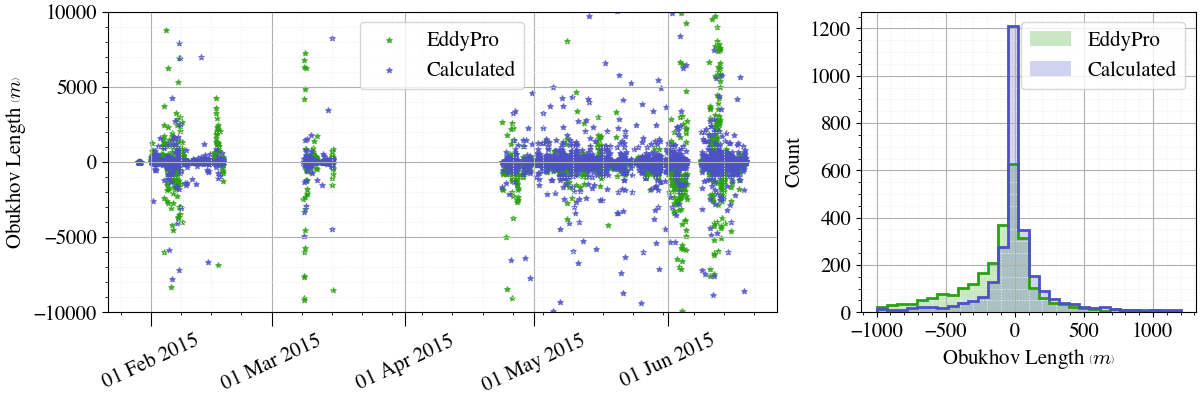
\includegraphics[width=1\linewidth]{figures/chapter5/ch3_obukhovlength.png}
    \caption[Obukhov length]{The Obukhov length measured during N-ICE and processed using EddyPro (green) and calculated using Eq. \ref{eq:l} (blue).}
    \label{fig:ol}
\end{figure}

The Obukhov length depends on the friction velocity, and the surface below N-ICE is first-year sea ice, a relatively flat surface with limited sources of mechanical turbulence. Friction velocity is a measure of the amount of wind shear \citep{stull:1988}. The mean friction velocity observed at N-ICE was 0.24 $m~s^{-1}$ with a standard deviation of approximately 0.1 $m~s^{-1}$. Friction velocity values from Eddypro were around 0.2 $m~s^{-1}$, with a maximum of about 1 $m~s^{-1}$. The results from EddyPro appear to represent a surface with more wind sheer than those calculated independently of EddyPro. 

\begin{table*}[t]
\centering
\footnotesize
\doublespacing
{
\begin{tabular}{| c | c | c | c | c | c | c |}
 \hline
\rowcolor[HTML]{F3F3F3} & \multicolumn{4}{c|}{\textbf{Mean Error $\left(W m^{-2}\right)$}} &  & \\
\rowcolor[HTML]{F3F3F3}  & \multicolumn{2}{c|}{\textbf{MEP}} & \multicolumn{2}{c|}{\textbf{Bulk}} & & \\
\rowcolor[HTML]{F3F3F3} \multirow{-3}{*}{\textbf{Author}} & $H_{l}$ & $H_{s}$ & $H_{l}$ & $H_{s}$ & \multirow{-3}{*}{\textbf{N}} & \multirow{-3}{*}{\shortstack{\textbf{Stability} \\ \textbf{Range}}} \\
 \hline
 Swainbank & 2.156 & -3.070  & -0.523 & -9.812 & 50 & $-2 \leq \zeta \leq -0.1$ \\ 
 Tschalikov & -1.054  & -7.556  & 0.559 & -63.357 & 312 & $0.04 \leq \zeta$ \\  
 Zilitinkevich and Tschalikov & 1.266 & -3.246 & -0.240  &  -2.065 & 1499 & $-1.2 < \zeta$ \\
 Businger et al. & 1.260 & -2.798  & -0.191 & 0.580 & 1475 & $-2 \leq \zeta$ \\
 Dyer &  1.468  & -2.327 & -0.325  & 7.871  & 1277 & $-1 \leq \zeta$ \\
 Skeib & 1.273 & -2.480  & -0.179 & 5.676  & 1422 & $-2 \leq \zeta \leq 2$ \\
 Gavrilov and Petrov & -0.294 & 2.307 & 0.111 & -28.549 & 1518 & all $\zeta$ \\
 Dyer and Bradley & 2.003  &  -6.299  & -0.511  & 14.959  & 814 & $0 \leq \zeta$ \\
 Beljaars and Holtslag &  -0.270 & 2.674 & 0.100 & 45.403 & 814 &  $0 \leq \zeta$ \\
 Handorf et al. & -0.274  &  2.508  & 0.133 & -39.040  & 814 & $ 0 \leq \zeta$ \\
 Andreas et al. & 0.617 & 0.882 & -0.175  & 5.071  & 1518 & all $\zeta$ \\
 \hline
\end{tabular}}
\caption[Sensible and latent heat flux mean error for each scaling function relationship.]{Mean error sensible and latent heat flux calculations using each scaling equation listed in Table \ref{tab:stability} for both the MEP equations and the bulk flux algorithm. The number of hourly measurements used and the applicable ranges are shown in the rightmost columns.}
\label{tab:stability_error}
\end{table*}

Table \ref{tab:stability_error} shows the mean error when using the MEP and bulk flux methods to calculate surface fluxes relative to the EddyPro results. Each source in the ``Author'' column corresponds to equations in Table \ref{tab:stability}. Each has a different number of hourly measurements included because each is applicable to specific ranges in stability. For example. Swainbank \citep{foken:2008} is only valid for surface-layer stability parameter values between -0.1 and -2, indicating this is only valid for unstable conditions, which we see rarely in the polar regions. So this formulation uses only a small number of observations for comparison. \citet{andreas:311}, on the other hand, was created using the SHEBA observations and has the largest range of value over which it is valid. The equations created by \citet{andreas:311} had the lowest mean error for the latent heat flux when using the MEP equation, however, its performance calculating the sensible heat flux was comparable to other equations considering the same wide range of stability values. 

Using the bulk flux algorithm resulted in similar errors for latent heat flux regardless of the scaling parameter relationship used with the exception of the Swainbank and Tschalikov \citep{foken:2008} formulations, which had a significantly lower and higher mean error, respectively. While Swainbank \citep{foken:2008} did have the lowest mean error for the latent heat flux and one of the lowest for the sensible heat flux, it was not selected for use because of the low number of stability conditions over which it can be used.  

Due to its wide range of stability values and its improved performance for latent heat flux, the \citet{andreas:2010} formulation was used for the final analysis of both the bulk flux equation and the MEP equation. The MEP equation typically uses the relations developed by \citet{businger:1971}, but for our location, the \citet{andreas:311} formulation performed better when compared to the EddyPro measurements when calculating latent heat flux. Sensible heat flux, on the other hand, was comparable between the \citet{andreas:311} formulation and the \citet{businger:1971} formulation. 

\subsection{Thermal Conductivity}
Thermal conductivity is used in the MEP method to calculate the thermal inertia parameter, as shown in Eq. \ref{eq:iwsi}. Thermal conductivity values at N-ICE were much lower than those commonly used in models \citep{merkouriadi:2017}, so special care was taken to ensure that the thermal conductivity estimate was accurate for our conditions. Using the thermal conductivity values shown in Table \ref{tab:thermal} with Eq. \ref{eq:iwsi}, the thermal inertia parameter was estimated for N-ICE as shown in Table \ref{tab:thermal}. 

\begin{table}[t]
\centering
\footnotesize
\doublespacing
{
\begin{tabular}{| c | c | c |}
 \hline
\rowcolor[HTML]{F3F3F3}  & \textbf{Thermal Conductivity} & \textbf{Thermal Inertia}\\
 \rowcolor[HTML]{F3F3F3}\multirow{-2}{*}{\textbf{Floe}} & $(m^{-1}K^{-1})$ & $(J~m^{-2}Ks^{-0.5})$ \\
  \hline
 1 & 314.264 & 0.183  \\
 2 & 429.650 & 0.246 \\ 
 3 & 280.424 & 0.193 \\
 4 & 1009.816 & 0.311 \\
  \hline
\end{tabular}}
\caption[Thermal conductivity and inertia.]{Thermal conductivity and inertia for each floe during N-ICE. Conductivity values were taken as a mean from \citet{merkouriadi:2017} and inertia parameters were calculated using equation \ref{eq:iwsi}.}
\label{tab:thermal}
\end{table}

\subsection{Bulk Flux Algorithm}
Calculating the fluxes using the bulk flux algorithm resulted in more large positive values than was seen in the EddyPro or in the MEP results. These can be seen in Figure \ref{fig:bulk:sensible}. In spring, the sensible heat flux is consistently over-estimated by the bulk flux algorithm, indicating that the temperature difference between the surface and the atmosphere is too large in the calculations, and too much heat is being transferred into the surface. The latent heat fluxes, shown in Figure \ref{fig:bulk:latent}, were also significantly larger than the EddyPro results when using the bulk flux algorithm. 

\begin{figure}[h!]
    \centering
    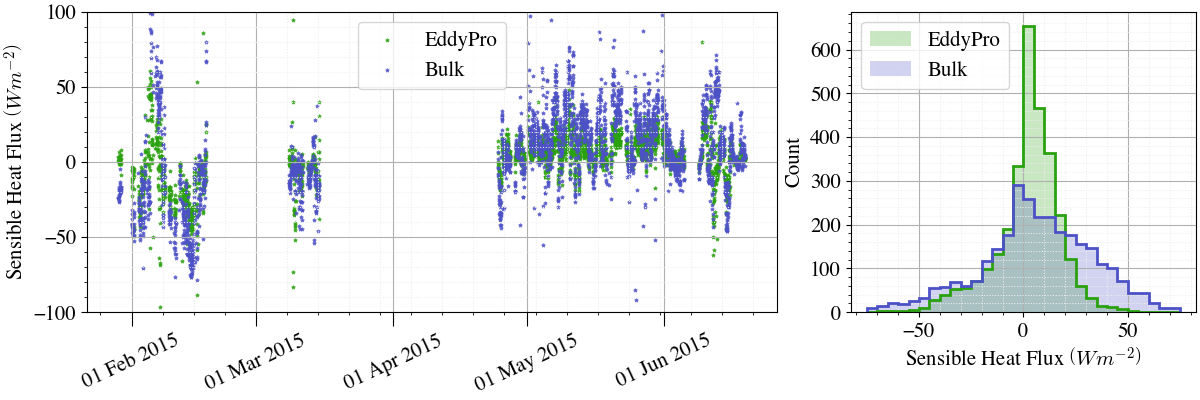
\includegraphics[width=1\linewidth]{figures/chapter5/BulkSensible.png}
    \caption[Sensible heat flux from a bulk flux method compared to EddyPro.]{The sensible heat flux at N-ICE as calculated with EddyPro (green) and with the bulk flux algorithm method (blue).}
    \label{fig:bulk:sensible}
\end{figure}
\begin{figure}[h!]
    \centering
    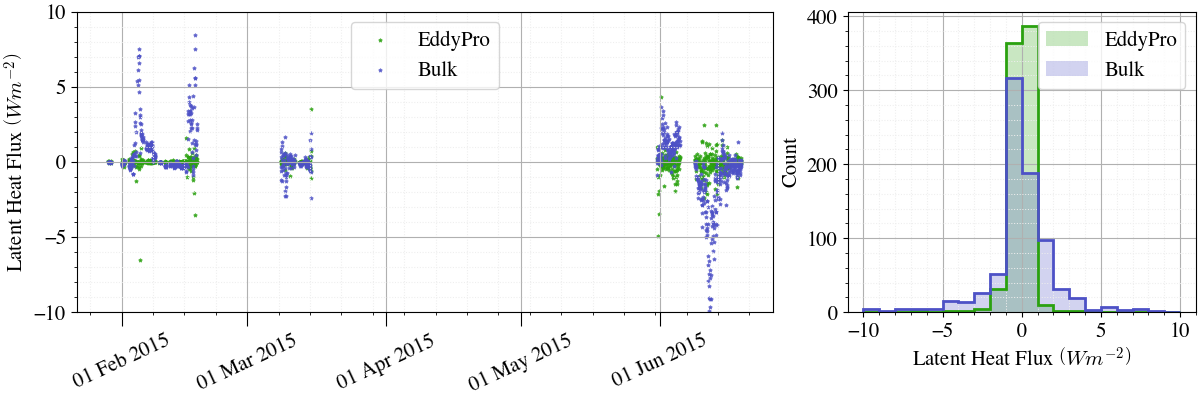
\includegraphics[width=1\linewidth]{figures/chapter5/BulkLatent.png}
    \caption[Latent heat flux from a bulk flux method compared to EddyPro.]{The latent heat flux at N-ICE as calculated with EddyPro (green) and with the bulk flux algorithm method (blue).}
    \label{fig:bulk:latent}
\end{figure}

In June, there was a large decrease in the latent heat flux according to the bulk algorithm. This was mirrored by an increase in the sensible heat flux. However, this decrease (increase) in the latent heat flux (sensible heat flux) was not seen in the EddyPro results. EddyPro produced latent heat flux values consistently around zero during this time period, while the sensible heat flux became negative. This indicates that the near-surface air was cooler than the surface and sensible heat transfer was occurring instead of a phase change. However, the bulk flux algorithm favored a phase change, likely melting, over a sensible heat flux change. At this time in the experiment, there likely was significant phase change occurring as many melt ponds were developing in the surrounding area \citep{walden:2017}. Overall, latent heat flux values estimated by the bulk equation are more largely positive in the winter and more largely negative in the summer, indicating the bulk flux algorithm shows more melting in the spring and more freezing in the winter than the EddyPro results. 

Positive latent heat flux values in the winter represent surface freezing. These values are, at times, almost 10 $Wm^{-2}$ greater in the bulk results than in the EddyPro results. EddyPro, once again, favors sensible heat flux changes to phase changes. However, the sensible heat flux in the bulk algorithm and in EddyPro are comparable. This indicates that EddyPro is not just favoring the heat transfer to be in the form of sensible heat flux, but it also underestimates the latent heat flux in general, even in situations when it cannot be described by an offset in the sensible heat flux. 

 \subsection{Maximum Entropy Method}
Sensible heat flux from the MEP method was calculated using Eq. \ref{eq:mep:hs}. The results of this are shown in Figure \ref{fig:mep:sensible}. For most of the experiment, the MEP method accurately represented the sensible heat fluxes at N-ICE. In the winter, fluxes were slightly underestimated by the MEP equation, resulting in a bi-modal shape to the distribution shown on the right of the figure. In the spring, there was one occurrence lasting several days with largely negative sensible heat flux shown in the EddyPro results while the sensible heat fluxes from the MEP equation were positive. 

\begin{figure}[h!]
    \centering
    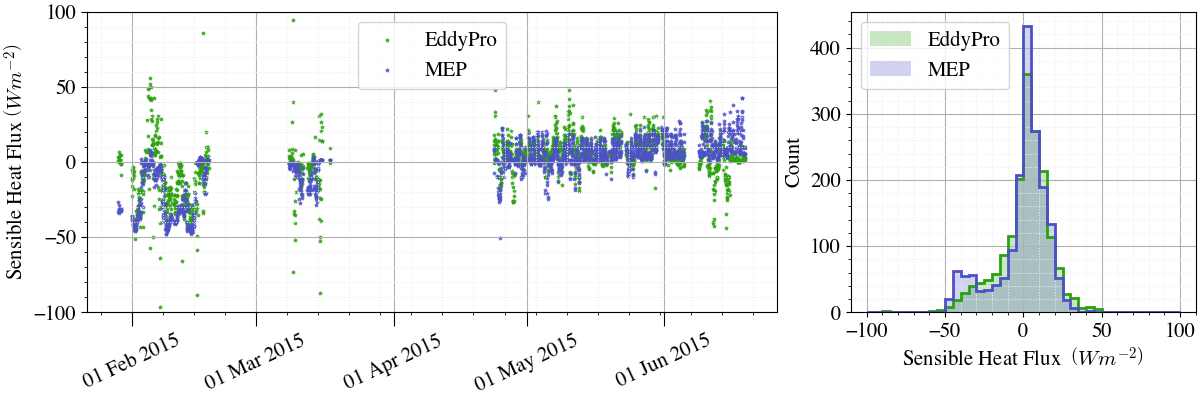
\includegraphics[width=1\linewidth]{figures/chapter5/MEPSensible.png}
    \caption[Sensible heat flux from the MEP method compared to EddyPro.]{The sensible heat flux at N-ICE as calculated with EddyPro (green) and with the MEP method (blue).}
    \label{fig:mep:sensible}
\end{figure}
\begin{figure}[h!]
    \centering
    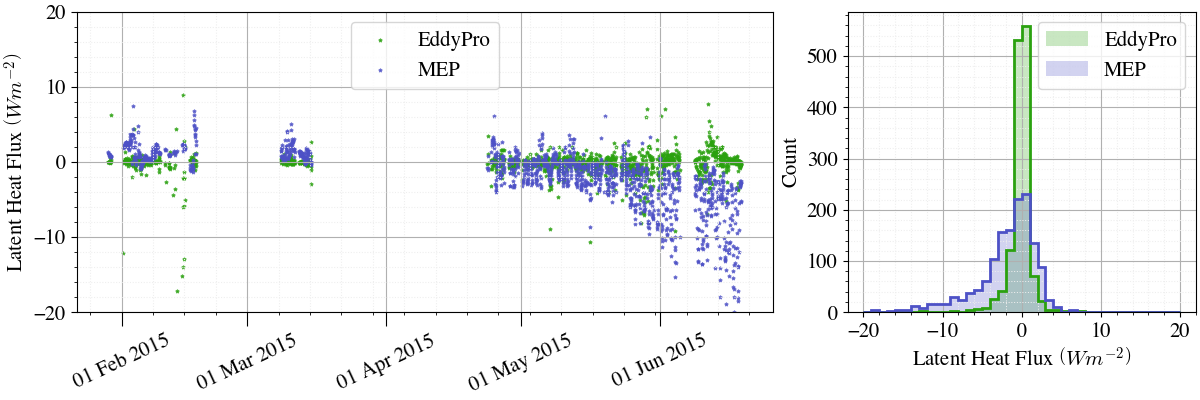
\includegraphics[width=1\linewidth]{figures/chapter5/MEPLatent.png}
    \caption[Latent heat flux from the MEP method compared to EddyPro.]{The latent heat flux at N-ICE as calculated with EddyPro (green) and with the MEP method (blue).}
    \label{fig:mep:latent}
\end{figure}

Latent heat fluxes (Figure \ref{fig:mep:latent}) were not represented as well using the MEP as compared to the EddyPro results. EddyPro showed very small latent heat fluxes throughout the entire experiment. These small heat fluxes were surprising and are not captured with the MEP method. February and March values of latent heat flux are comparable between the MEP and EddyPro calculations, but during spring and entering summer, MEP values are at times 20 $Wm^{-2}$ greater than those calculated by EddyPro, which are rarely greater than 10 $Wm^{-2}$.

\section{Conclusions}
Sensible and latent heat flux formulations require high temporal resolution to use eddy covariance methods. Two methods of calculating sensible and latent heat flux that do not require eddy covariance measurements are explored here. The MEP method is a method utilizing thermal conductivity, net radiative flux, and stability. The bulk flux method requires measurements of moisture and temperature, wind speed, and stability at two levels near the surface. Both equations require the bulk transfer coefficients of heat and moisture, which are a function of stability and have been empirically defined for experiments over a variety of surfaces. Very few of these functions are appropriate for the strong stability conditions that often occur in polar regions. \citet{andreas:311} developed a relationship for these functions that applies to strong stability using data from SHEBA over multi-year sea ice. This relationship was also found to be appropriate for the bulk transfer coefficients at N-ICE using both the bulk flux method and the MEP method. 

The MEP method performed well when compared to the EddyPro values for both sensible and latent heat fluxes. In the winter, the latent heat flux values calculated by the MEP equation are much higher than those in EddyPro, indicating  more phase change. The bulk method also represented the EddyPro values fairly well, although the MEP formulations seem to represent the spread of flux values better than the bulk algorithm. The latent heat flux values were also much larger than those observed during N-ICE in the bulk method. 

Overall, further testing is needed for the validation of the latent heat flux formulations. The latent heat flux values measured at N-ICE were much smaller than expected and smaller than those seen in other experiments, so more measurements are needed to rule out any issue with the N-ICE observations. Both sensible heat flux formulations, however, produced reasonable values over the first-year sea ice seen at N-ICE. 



